%%
%% This is file `sample-sigconf.tex',
%% generated with the docstrip utility.
%%
%% The original source files were:
%%
%% samples.dtx  (with options: `sigconf')
%% 
%% IMPORTANT NOTICE:
%% 
%% For the copyright see the source file.
%% 
%% Any modified versions of this file must be renamed
%% with new filenames distinct from sample-sigconf.tex.
%% 
%% For distribution of the original source see the terms
%% for copying and modification in the file samples.dtx.
%% 
%% This generated file may be distributed as long as the
%% original source files, as listed above, are part of the
%% same distribution. (The sources need not necessarily be
%% in the same archive or directory.)
%%
%%
%% Commands for TeXCount
%TC:macro \cite [option:text,text]
%TC:macro \citep [option:text,text]
%TC:macro \citet [option:text,text]
%TC:envir table 0 1
%TC:envir table* 0 1
%TC:envir tabular [ignore] word
%TC:envir displaymath 0 word
%TC:envir math 0 word
%TC:envir comment 0 0
%%
%%


%% The first command in your LaTeX source must be the \documentclass command.
\documentclass[sigconf]{acmart}


%%
%% \BibTeX command to typeset BibTeX logo in the docs
\AtBeginDocument{%
  \providecommand\BibTeX{{%
    \normalfont B\kern-0.5em{\scshape i\kern-0.25em b}\kern-0.8em\TeX}}}

%% Rights management information.  This information is sent to you
%% when you complete the rights form.  These commands have SAMPLE
%% values in them; it is your responsibility as an author to replace
%% the commands and values with those provided to you when you
%% complete the rights form.
% TODO
\setcopyright{acmcopyright}
\copyrightyear{2023}
\acmYear{2023}
\acmDOI{10.1145/1122445.1122456}

%% These commands are for a PROCEEDINGS abstract or paper.
% TODO:
\acmConference[GECCO 2023]{Genetic
and Evolutionary Computation Conference Companion}{2023}{Portugal}
% \acmConference[Woodstock '18]{Woodstock '18: ACM Symposium on Neural
%   Gaze Detection}{June 03--05, 2018}{Woodstock, NY}
% \acmBooktitle{Woodstock '18: ACM Symposium on Neural Gaze Detection,
%   June 03--05, 2018, Woodstock, NY}
% \acmPrice{15.00}
% \acmISBN{978-1-4503-XXXX-X/18/06}


%%
%% Submission ID.
%% Use this when submitting an article to a sponsored event. You'll
%% receive a unique submission ID from the organizers
%% of the event, and this ID should be used as the parameter to this command.
%%\acmSubmissionID{123-A56-BU3}

%%
%% The majority of ACM publications use numbered citations and
%% references.  The command \citestyle{authoryear} switches to the
%% "author year" style.
%%
%% If you are preparing content for an event
%% sponsored by ACM SIGGRAPH, you must use the "author year" style of
%% citations and references.
%% Uncommenting
%% the next command will enable that style.
%%\citestyle{acmauthoryear}

\usepackage{annotate-equations}
\usepackage{xcolor}
\usepackage{algorithm}
\usepackage{algpseudocode}

\definecolor{ForestGreen}{HTML}{009B55}
\definecolor{MidnightBlue}{HTML}{006795}
% \definecolor{ForestGreen}{HTML}{009B55}

\renewcommand{\algorithmicrequire}{\textbf{Input:}}
\renewcommand{\algorithmicensure}{\textbf{Output:}}

\usepackage{tabularx, environ}

\makeatletter

% https://tex.stackexchange.com/a/199244/26355
\newcolumntype{\expand}{}
\long\@namedef{NC@rewrite@\string\expand}{\expandafter\NC@find}

\NewEnviron{problem}[2][]{%
  \def\problem@arg{#1}%
  \def\problem@framed{framed}%
  \def\problem@lined{lined}%
  \def\problem@doublelined{doublelined}%
  \ifx\problem@arg\@empty%
    \def\problem@hline{}%
  \else%
    \ifx\problem@arg\problem@doublelined%
      \def\problem@hline{\hline\hline}%
    \else%
      \def\problem@hline{\hline}%
    \fi%
  \fi%
  \ifx\problem@arg\problem@framed%
    \def\problem@tablelayout{|>{\bfseries}lX|c}%
    \def\problem@title{\multicolumn{2}{|%
      >{\raisebox{-\fboxsep}}%
      p{\dimexpr\columnwidth-4\fboxsep-2\arrayrulewidth\relax\rule{0pt}{4ex}\hspace{-1em}}%
      |}{%
        \textsc{\Large #2}%
      }}%
  \else
    \def\problem@tablelayout{>{\bfseries}lXc}%
    \def\problem@title{\multicolumn{2}{>%
      {\raisebox{-\fboxsep}}%
      p{\dimexpr\columnwidth-4\fboxsep\relax\rule{0pt}{3ex}\hspace{-1em}}%
      }{%
        \textsc{\Large #2}%
      }}%
  \fi%
  \bigskip\par\noindent%
  \renewcommand{\arraystretch}{1.2}%
  \begin{tabularx}{\columnwidth}{\expand\problem@tablelayout}%
    \problem@hline%
    \problem@title\\[2\fboxsep]%
    \BODY\\\problem@hline%
  \end{tabularx}%
  \medskip\par%
}
\makeatother


%%
%% end of the preamble, start of the body of the document source.
\begin{document}

%%
%% The "title" command has an optional parameter,
%% allowing the author to define a "short title" to be used in page headers.
\title{Calculating selection probabilities under lexicase selection is NP-Hard}

%%
%% The "author" command and its associated commands are used to define
%% the authors and their affiliations.
%% Of note is the shared affiliation of the first two authors, and the
%% "authornote" and "authornotemark" commands
%% used to denote shared contribution to the research.

\author{Emily Dolson}
 \email{dolsonem@msu.edu}
 \orcid{0000-0001-8616-4898}
 \affiliation{%
   \institution{Michigan State University}
   \city{East Lansing}
   \state{Michigan}
   \country{USA}
 }

%%
%% By default, the full list of authors will be used in the page
%% headers. Often, this list is too long, and will overlap
%% other information printed in the page headers. This command allows
%% the author to define a more concise list
%% of authors' names for this purpose.
\renewcommand{\shortauthors}{Dolson}

%%
%% The abstract is a short summary of the work to be presented in the
%% article.
\begin{abstract}
 % TODO
\end{abstract}

%%
%% The code below is generated by the tool at http://dl.acm.org/ccs.cfm.
%% Please copy and paste the code instead of the example below.
%%

\begin{CCSXML}
<ccs2012>
   <concept>
       <concept_id>10003752.10003809.10011254.10011255</concept_id>
       <concept_desc>Theory of computation~Backtracking</concept_desc>
       <concept_significance>100</concept_significance>
       </concept>
   <concept>
       <concept_id>10003752.10003809.10011254.10011256</concept_id>
       <concept_desc>Theory of computation~Branch-and-bound</concept_desc>
       <concept_significance>100</concept_significance>
       </concept>
   <concept>
       <concept_id>10003752.10003777.10003779</concept_id>
       <concept_desc>Theory of computation~Problems, reductions and completeness</concept_desc>
       <concept_significance>500</concept_significance>
       </concept>
   <concept>
       <concept_id>10003752.10003777.10003778</concept_id>
       <concept_desc>Theory of computation~Complexity classes</concept_desc>
       <concept_significance>500</concept_significance>
       </concept>
   <concept>
       <concept_id>10010147.10010257.10010293.10011809.10011813</concept_id>
       <concept_desc>Computing methodologies~Genetic programming</concept_desc>
       <concept_significance>500</concept_significance>
       </concept>
 </ccs2012>
\end{CCSXML}

\ccsdesc[500]{Theory of computation~Problems, reductions and completeness}
\ccsdesc[500]{Theory of computation~Complexity classes}
\ccsdesc[500]{Computing methodologies~Genetic programming}
\ccsdesc[100]{Theory of computation~Backtracking}
\ccsdesc[100]{Theory of computation~Branch-and-bound}

%%
%% Keywords. The author(s) should pick words that accurately describe
%% the work being presented. Separate the keywords with commas.
\keywords{lexicase selection, NP-Completeness, selection probabilities}

%% A "teaser" image appears between the author and affiliation
%% information and the body of the document, and typically spans the
%% page.
% TODO (optionally)
% \begin{teaserfigure}
%   \includegraphics[width=\textwidth]{sampleteaser}
%   \caption{Seattle Mariners at Spring Training, 2010.}
%   \Description{Enjoying the baseball game from the third-base
%   seats. Ichiro Suzuki preparing to bat.}
%   \label{fig:teaser}
% \end{teaserfigure}

%%
%% This command processes the author and affiliation and title
%% information and builds the first part of the formatted document.
\maketitle

\section{Introduction}

% Lexicase selection is very good 
% It is tempting to try to calculate probabilities of selection under lexicase and use those
% It would also be handy to be able to calculate them for various theoretical purposes
% So it would be useful to know if it's possible to do so efficiently

% Turns out it's not
% Here we show that lexicase is NP-Hard by reduction from Satisfiability
% Also applies to epsilon lexicase because we can trivially reduce lexicase to epsilon lexicase

Lexicase selection is a state-of-the-art technique for selecting parents to reproduce in genetic programming \citep{spector_assessment_2012} [ADD MORE CITATIONS HERE]. It is also increasingly being successfully applied in evolutionary computation domains outside of genetic programming \citep{metevier_lexicase_2019}. Consequently, it would be valuable to develop a more rigorous theoretical understanding of lexicase selection, what makes it so effective, and what its limitations are. Most theoretical analyses of lexicase selection to date have involved calculating the probability of a given individual being selected on a given selection event \citep{la_cava_probabilistic_2018, dolson_ecological_2018}. This value, referred to as $P_{lex}$ in \citep{la_cava_probabilistic_2018}, is critical to determining the long-term outcome of lexicase selection. 

This analysis is impeded by the fact that the naive approach to calculating $P_{lex}$ has exponential run time \citep{la_cava_probabilistic_2018}. Various optimizations can be applied to dramatically improve this run-time in practice, which makes it tempting to believe that calculating $P_{lex}$ in polynomial time might be possible. The creation of a polynomial time algorithm for calculating $P_{lex}$ would facilitate more advanced theoretical analyses and potentially open up new avenues for refining lexicase selection. For example, \citep{la_cava_probabilistic_2018} points out that it would be tempting to plug $P_{lex}$ into a roulette selection algorithm as a potential simplification to the algorithm if calculating it were not so expensive in terms of run time.

However, thus far no one has succeeded at developing a polynomial time algorithm for calculating $P_{lex}$. Is doing so likely to be possible? Here, we show that it is not, by proving that the problem of calculating $P_{lex}$ is $NP$-Hard. These results extend to calculating $P_{lex}$ for other lexicase selection variants such as $\epsilon$-lexicase [CITE], downsampled lexicase \citep{hernandez_random_2019,ferguson_characterizing_2020}, and [ONE MORE].

\section{Background}

\subsection{Lexicase Selection}

Lexicase selection is designed to operate in contexts in which candidate solutions in a population are evaluated on multiple fitness criteria. In genetic programming, for example, these fitness criteria are often test cases that a program may be evaluated on. It is common to use a large number of fitness criteria (i.e. hundreds). Rather than combining a candidate solution's performance on each criterion into a single score, lexicase selection considers each one individually. 

To select a candidate solution to reproduce under lexicase selection, a random fitness criterion is chosen. All but the top-performing candidate solutions on that criterion are eliminated from consideration for selection. Then another random fitness criterion is chosen. Out of the set of solutions that were still in contention for selection, all but best performers on this new criterion are then eliminated. This process continues until either only one candidate solution remains, at which point that candidate is chosen to reproduce. If all fitness criteria have been used and there are still multiple candidate solutions remaining, one of them is selected randomly. For a more in-depth explanation with examples, see \citep{spector_assessment_2012, la_cava_probabilistic_2018}.

\begin{algorithm}
\caption{The Lexicase selection algorithm}\label{alg:cap}
\begin{algorithmic}
\Require P - a vector of $N$ candidate solutions, each represented as a vector of scores on $M$ fitness criteria 
\Ensure A single candidate solution from P that should reproduce
\State $F \gets 1...M$ \Comment{Set of fitness criteria to consider}
\State $S \gets P$ \Comment{Set of candidate solutions to consider}
\While{$|P| > 1$ \& $|F| > 0$}
\State curr $\gets$ random criterion in $F$
\State best $\gets$ -1 \Comment{Assumes fitness is being maximized}
\For{solution : $S$}
\If{solution[curr] > best}
\State best $\gets$ solution[curr]
\EndIf
\EndFor
\State $S \gets$ all members of $S$ with score best on criterion curr
\EndWhile

\hspace{-2em}\Return{A random candidate solution in $S$}
\end{algorithmic}
\end{algorithm}

\subsection{$\epsilon$-Lexicase Selection}

A number of variations on the core concept of lexicase selection have been developed. The most relevant to this paper is $\epsilon$-Lexicase Selection, which is commonly used when fitness criteria are floating point numbers [CITE]. This variation adds a parameter, $\epsilon$, which provides a margin for error in the identification of the top performers on a given fitness criterion. In traditional lexicase selection, candidate solutions must be tied for best on the current fitness criterion in order to remain in contention for selection. In $\epsilon$-lexicase selection, however, candidate solutions need only be within $\epsilon$ of the best score on the current fitness criterion to remain in contention.

%\subsection{Other Lexicase Variants}
 %TODO: Write this if neceessary


\section{Preliminaries}

\subsection{Problem Definitions}

There are five problems that it is important to formally define for the purposes of the following proofs. The first is the problem of calculating selection probabilities under lexicase selection ($P_{lex}$. We will call this problem the {\sc Lexicase Selection Probabilities Problem}, and will abbreviate it as {\sc lex-prob}. It is formally defined as follows:

\begin{problem}[ruled]{Lexicase Selection Probabilities Problem (lex-prob)}
  Input: & 1) a two-dimensional vector, $P$, containing $N$ vectors of length $M$. Each of the $N$ vectors represents a candidate solution in the population, and the values in the vector represent that solution's scores on each of the $M$ fitness criteria; 2) an integer $i$ indicating the index of a vector in $P$ \\
  Output: & The probability that vector $i$ would be selected from population $P$ by lexicase selection ($P_{lex_i}$)\\
\end{problem}

Note that this definition applies to calculating the selection probability for a single member of the population. In many cases, it is desirable to calculate selection probabilities for all members of a population. In practice, there are substantial efficiency gains from calculating probabilities for all members of the population at the same time. However, because the problem of calculating the probability of selection for a single member of the population is strictly easier, we will focus on it; if we prove that calculating $P_{lex}$ for even a single member of the population is $NP$-Hard, that will trivially show that calculating $P_{lex}$ for the entire population is also $NP$-Hard. Indeed, both versions of this problem can be reduced to each other in polynomial time\footnote{Calculating $P_{lex}$ for the entire population can be achieved by calculating $P_{lex}$ for each individual member of the population (i.e. $N$ times). Conversely, calculating $P_{lex}$ for an individual can be achieved by calculating it for the whole population and examining the value for that individual.} and thus they must be in the same complexity class. 

When proving that problems are $NP$-Hard, it is often easier to work with the \textit{decision} version of a problem, i.e. a version of the problem that returns a Boolean True or False as an answer. We define the decision version of {\sc lex-prob} as follows: 

\begin{problem}[ruled]{Decision Version of lex-prob}
  Input: & same as {\sc lex-prob}\\
  Output: & A Boolean value indicating whether there is a non-zero probability that vector $i$ would be selected from population $P$ by lexicase selection ($P_{lex_i}$)\\
\end{problem}

Note that, as is typically the case with decision versions of problems, the full version of {\sc lex-prob} trivially reduces to the decision version; output from the full version can trivially be converted to output for the decision version by comparing the returned $P_{lex}$ value to 0. Consequently, the full version can only be harder than the decision version, and so proving the decision version to be $NP$-Hard also proves the full version to be $NP$-Hard.

We will also use the $\epsilon$-Lexicase Selection Probabilities Problem (abbreviated as {\sc $\epsilon$-lex-prob}) as a step in our proof. {\sc $\epsilon$-lex-prob} is the problem of calculating $P_{lex}$ under $\epsilon$ lexicase selection. It is formally defined as follows:

\begin{problem}[ruled]{$\epsilon$-Lexicase Selection Probabilities Problem ($\epsilon$-lex-prob)}
  Input: & All of the inputs to {\sc lex-prob}, plus a floating point value, $\epsilon$, indicating the allowed margin of error for selecting elite candidate solutions on each fitness criterion\\
  Output: & The probability that vector $i$ would be selected from population $P$ by $\epsilon$-lexicase selection ($P_{\epsilon-lex_i}$) using the specific $\epsilon$ value\\
\end{problem}

As with {\sc lex-prob}, we will primarily use the decision version of {\sc $\epsilon$-lex-prob} in our proof. Like {\sc lex-prob}, {\sc $\epsilon$-lex-prob} can trivially be reduced to its decision version, meaning the full {\sc $\epsilon$-lex-prob} problem must be as hard as or harder than its decision version. We formally define the decision version of {\sc $\epsilon$-lex-prob} as follows:

\begin{problem}[ruled]{Decision version of $\epsilon$-lex-prob}
  Input: & same s {\sc $\epsilon$-lex-prob}\\
  Output: & A Boolean value indicating whether there is a non-zero probability that vector $i$ would be selected from population $P$ by $\epsilon$-lexicase selection ($P_{\epsilon-lex_i}$) using the specific $\epsilon$ value\\
\end{problem}

To prove that {\sc lex-prob} is $NP$-Hard, one must show that some problem that is already known to be $NP$-Hard can be reduced to {\sc lex-prob} in polynomial time. Thus, we must select a known $NP$-Hard problem to use as a starting point. Here, we will use the classic $NP$-Hard problem, {\sc Boolean Satisifiability} (commonly abbreviated as {\sc SAT}) [CITE], which is defined as follows:

\begin{problem}[ruled]{Boolean Satisfiability (SAT)}
  Input: & 1) a set, $V$, of $n$ variables, and 2) a set, $C$, of $m$ clauses containing variables in $V$ or their negations\\
  Output: & A Boolean value indicating whether it is possible to assign truth values (i.e. True or False) to each variable in $V$ such that each clause in $C$ contains at least one element that evaluates to True. \\
\end{problem}


\subsection{Brief review of computational complexity theory}

For readers unfamiliar with the $NP$-Hard class of problems and how we prove that problems are in this class, we offer a capsule summary. 

In order to talk about how hard problems are, we place them into classes. Many problems that we regularly encounter are in the class $NP$ (non-deterministically polynomial), which is the set of problems for which we can verify in polynomial time that a given solution is correct. Some problems in $NP$ are ``easy'' in the sense that polynomial-time solutions for them have been found. For the hardest problems in $NP$, no polynomial-time solution has been found thus far and it is thought to be unlikely that one exists. $NP$-Hard problems are the class of problems that are at least as hard as the hardest problems in $NP$. Thus, if a problem is $NP$-Hard, it is unlikely to be solvable in polynomial time. If calculating lexicase selection probabilities is $NP$-Hard, that is useful to know because it tells us that efforts to find a polynomial time algorithm to calculate them are unlikely to pay off.

To prove that a problem is $NP$-Hard, we must take a problem that we already know is $NP$-Hard show that it reduces (in polynomial time) to the problem we're interested in.  Here, we will reduce {\sc SAT} to {\sc $\epsilon$-lex-prob}, i.e. we will convert instances of {\sc SAT} to instances of {\sc $\epsilon$-lex-prob} that, when solved, will also tell us the solution to the underlying {\sc SAT} instance. By showing that any instance of {\sc SAT} can be converted to an equivalent instance of {\sc $\epsilon$-lex-prob} in polynomial time, we will prove that {\sc $\epsilon$-lex-prob} is at least as hard as {\sc SAT}. If we came up with a polynomial time algorithm that solved {\sc $\epsilon$-lex-prob}, that would mean we also have a polynomial time algorithm for {\sc SAT} (and, indeed, all of the $NP$-Complete problems). As the suspicion of most experts is that {\sc SAT} cannot be solved in polynomial time [CITE], this would mean that {\sc $\epsilon$-lex-prob} likely cannot be solved in polynomial time either. We will subsequently show that {\sc $\epsilon$-lex-prob} reduces in polynomial time to {\sc lex-prob}, and thus {\sc lex-prob} is, by the same logic, also $NP$-Hard.

Some readers may be more familiar with the class $NP$-Complete. $NP$-Complete problems are problems that are $NP$-Hard and are also in the set $NP$. Typically, only the decision versions of problems are $NP$-Complete, as verifying that the precise values returned by non-decision problems is seldom easier than calculating them in the first place. While we will show that the decision versions of {\sc $\epsilon$-lex-prob} and {\sc lex-prob} are $NP$-Complete, the emphasis of this paper is on the full versions of the problems. As these problems seem unlikely to be in $NP$, we have chosen to emphasize that the full versions are $NP$-Hard, rather than that the decision versions are $NP$-Complete. Both of those statements are true, however, and both imply that creating a polynomial time solution to any of these problems is unlikely to be possible.

\section{{\sc lex-prob} and {\sc $\epsilon$-lex-prob} are $NP$-Hard}

We will prove that {\sc lex-prob} and {\sc $\epsilon$-lex-prob} are $NP$-Hard via the following sequence of reductions:

\[
\text{{\sc SAT}} \leq_{P} \text{{\sc $\epsilon$-lex-prob} (decision)} \leq_{P} \text{{\sc lex-prob} (decision)}
\]

In other words, we will show that {\sc SAT}, a known $NP$-Hard problem, can be reduced in polynomial time to the {\sc $\epsilon$-lex-prob} problem. Subsequently, we will show that the {\sc $\epsilon$-lex-prob} problem can be reduced in polynomial time to the {\sc lex-prob} problem. For convenience, we will use the decision version of {\sc $\epsilon$-lex-prob} and {\sc lex-prob}. As the decision versions of each trivially reduce in polynomial time to the full versions, this series of reductions will prove that both versions of these problems are $NP$-Hard. Formally:

\[
\text{{\sc SAT}} \leq_{P} \text{{\sc $\epsilon$-lex-prob} (decision)} \leq_{P} \text{{\sc $\epsilon$-lex-prob}}
\]
\[
\text{and}
\]
\[
\text{{\sc $\epsilon$-lex-prob} (decision)} \leq_{P} \text{{\sc lex-prob} (decision)} \leq_{P} \text{{\sc lex-prob}}
\]

We will also prove that the decision versions of {\sc $\epsilon$-lex-prob} and {\sc lex-prob} are $NP$-Complete by showing that, in addition to being $NP$-Hard, these problems are in $NP$.

\subsection{The decision versions of {\sc lex-prob} and {\sc $\epsilon$-lex-prob} are in $NP$}

In order to show that the decision version of {\sc lex-prob} and {\sc $\epsilon$-lex-prob} are $NP$-Complete, we must first show that they are in $NP$.

\begin{theorem}
\label{np_theorem}
{\sc lex-prob} and {\sc $\epsilon$-lex-prob} are in the set $NP$.
\end{theorem}

In the formal definition of a decision problem, its only output is True or False. However, for the purposes of demonstrating membership in the class $NP$, it is also allowed to return additional information (a ``certificate'') for use in verifying that the True/False output is correct. 

\begin{proof}
    Let the certificate returned by {\sc lex-prob} or {\sc $\epsilon$-lex-prob} be a list, $L$, denoting an order in which fitness criteria could be selected that would cause candidate solution $i$ to be selected by lexicase selection or $\epsilon$-lexicase selection.

    The size of $L$ will be $\mathcal{O}(M)$, where $M$ is the number of fitness criteria.

    To verify that the returned answer is correct, we simply need to step through the fitness criteria in the order specified by $L$, removing individuals from the original population, $P$, according to the rules of lexicase selection. This process can be carried out in $\mathcal{O}(MN)$ time, where $N$ is the number of candidate solutions in the population.

    As $MN$ is a polynomial, this verification can be carried out in polynomial time and {\sc lex-prob} and {\sc $\epsilon$-lex-prob} are both in $NP$.
\end{proof}

Note that the full versions of {\sc $\epsilon$-lex-prob} and {\sc lex-prob} do not appear to be in the set $NP$, because there is no obvious polynomial-sized certificate that could be returned that would allow the correctness of the assigned probabilities to be verified. 

\subsection{{\sc $\epsilon$-lex-prob} is $NP$-Hard}

\begin{figure*}
    \centering
    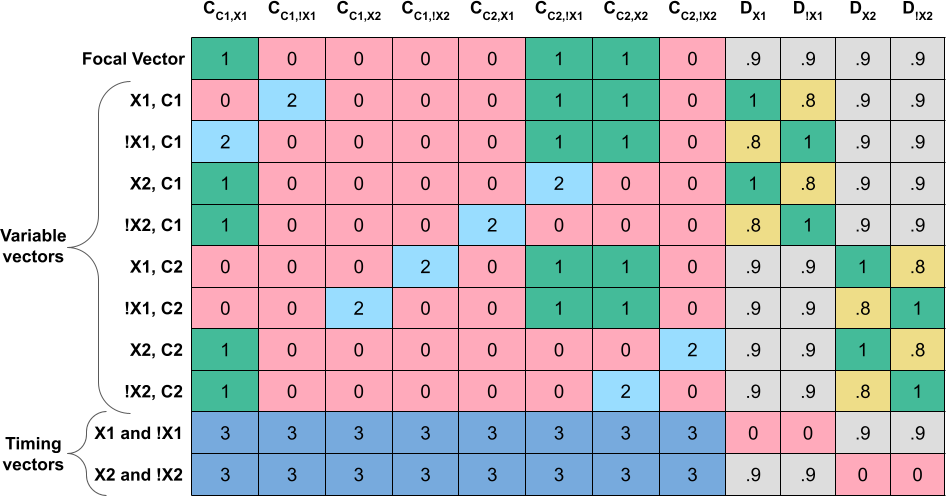
\includegraphics[width=\linewidth]{figs/SAT_to_eps_example.png}
    \caption{Worked example of reducing {\sc SAT} to {\sc $\epsilon$-lex-prob}. This is the {\sc $\epsilon$-lex-prob} instance corresponding to the {\sc SAT} following instance: $V = \{X1, X2\}$, $C = \{X1\}, \{!X1, X2\}$}
    \label{fig:sat_to_eps}
\end{figure*}

We propose the following theorem:

\begin{theorem}
\label{elexicasetheorem}
{\sc $\epsilon$-lex-prob} is $NP$-Hard.
\end{theorem}

We will prove this theorem by reducing Satisfiability ({\sc SAT}), a well-known $NP$-Complete problem [CITE Karp], to the decision version of {\sc $\epsilon$-lex-prob} in polynomial time. For a worked example of this reduction, see Figure \ref{fig:sat_to_eps}.

\begin{proof}
Given an instance of {\sc SAT} with $c$ clauses and $v$ variables, we can create an instance of {\sc $\epsilon$-lex-prob} with a population, $P$, containing $N = 1 + 2vc + v$ candidate solutions with scores on $M = 2vc + 2v$ fitness criteria. $P$ can be visualized as a matrix where row vectors are candidate solutions and column vectors are fitness criteria. $\epsilon$ will be set to .1. 

The first $2vc$ fitness criteria in each candidate solution correspond to the clauses in the original {\sc SAT} instance. The representation of each clause is made up of $2v$ fitness criteria, one for each variable and the negation of each variable. We will refer to these fitness criteria as $C_{C_{i},X_{j}}$, where $i$ is the index of the clause the fitness criterion is part of and $j$ is the id of the variable the fitness criterion refers to. For example, $C_{C2X3}$ would be the criterion corresponding to the value of the variable $X3$ in clause 2.

The next $2v$ fitness criteria are the ones that will be used to explore different assignments of truth values to variables in the {\sc SAT} instance. The order in which lexicase selection picks these fitness criteria will determine which variable assignments are made. We will refer to the position corresponding to choosing to set $Xi$ to true as $D_{Xi}$ (whereas the position that corresponds to setting it to false would be $D_{!Xi}$).

The first candidate solution in $P$, which we term the \textit{focal vector}, directly represents the {\sc SAT} instance. Its scores on the $C_{C_{i},X_{j}}$ fitness criteria will be set to indicate which variables are in each clause. If clause $i$ contains variable $j$, then $C_{C_{i},X_{j}}$ in the focal vector is set to 1. Otherwise, it is set to 0. All $D_{Xi}$ values are set to .9. The rules for creating the focal vector are stated formally in equation \ref{eq:focal_vector}.
\vspace{1.5em}

\begin{equation}
\label{eq:focal_vector}
\eqnmarkbox[violet]{fvi}{FV(x)} = \begin{cases} 
1 & \eqnmarkbox[teal]{ccixj}{x < 2cv} \text{ } \& \eqnmarkbox[blue]{var_xj}{X_{x\%(2v)}} \in \eqnmarkbox[magenta]{clause_ci}{C_{\lfloor i/(2v)\rfloor}} \\
0 & \eqnmarkbox[teal]{ccixj2}{i < 2cv} \text{ } \& \eqnmarkbox[blue]{var_xj2}{X_{x\%(2v)}} \notin \eqnmarkbox[magenta]{clause_ci2}{C_{\lfloor x/(2v)\rfloor}} \\
.9 & \eqnmarkbox[red]{dxi}{\text{otherwise}}
\end{cases}
\end{equation}

\annotate[yshift=1em]{left}{ccixj}{$x$ is a $C_{C_{i},X_{j}}$ criterion}
\annotate[yshift=1em]{right}{var_xj}{this criterion's variable ($X_j$) }
\annotate[yshift=-.2em]{below, right}{clause_ci2}{this criterion's \\ \sffamily\footnotesize clause ($C_i$)}
\annotate[yshift=-2.8em]{below,right}{fvi}{$x$th value of focal vector}
\annotate{below,right}{dxi}{$D_{Xi}$ objectives}
\vspace{1.5em}

The next $2vc$ candidate solutions in the population correspond to possible variable assignments for each clause. We will call these the \textit{variable vectors}. Let variable vector $VV_{ab}$ be the variable vector corresponding to clause $C_a$ and variable $X_b$. The $C_{C_{i},X_{j}}$ criteria values for $VV_{ab}$ are identical to the focal vector's, except for when $i=a$ (i.e. in the clause corresponding to $VV_{ab}$). $VV_{ab}$'s scores for all such fitness criteria ($C_{CaXj}$) will be 0, except when $j=inv(b)$. $VV_{ab}$ score for this fitness criterion, $C_{Ca!Xb}$, which corresponds to the negation of variable $Xb$ in clause $a$, will be set to 2. 

$D_{Xi}$ values for the variable vectors are set to .9, except in the position corresponding to that variable and its negation. For variable vectors corresponding to $Xi$, $D_{!Xi}$ will be set to .8, and $D_{Xi}$ will be set to 1. For variable vectors corresponding to $!Xi$, $D_{!Xi}$ will be set to 1, and $D_{Xi}$ will be set to .8. The rules for creating the focal vector are stated formally in equation \ref{eq:variable_vector}.

\vspace{3em}

\begin{equation}
\label{eq:variable_vector}
\eqnmarkbox[violet]{vvi}{VV_{xy}(z)} = \begin{cases} 
2 & \eqnmarkbox[teal]{ccixj2}{z < 2cv} \text{ } \& \eqnmarkbox[blue]{clausei}{x = {\lfloor z/(2v)\rfloor}}  \text{ } \& \eqnmarkbox[magenta]{inv_var}{\text{ inv}(y) = z\%(2v)}\\
0 & \eqnmarkbox[teal]{ccixj}{z < 2cv} \text{ } \& \eqnmarkbox[blue]{clausei2}{x = {\lfloor z/(2v)\rfloor}}  \text{ } \& \text{ inv}(y) \neq z\%(2v)\\
FV_z & \eqnmarkbox[teal]{ccixj}{z < 2cv} \text{ } \& x \neq {\lfloor z/(2v)\rfloor} \\
1 & \eqnmarkbox[orange]{dxi1}{z \geq 2cv \text{ } \& \text{ } z - 2cv = y}  \\
.8 & \eqnmarkbox[gray]{dxi3}{z \geq 2cv \text{ } \& \text{ } z - 2cv = inv(y)}  \\
.9 & \eqnmarkbox[red]{dxi2}{\text{otherwise}}
\end{cases}
\end{equation}

\annotate[yshift=1em]{left}{ccixj2}{$k$ is a $C_{C_{i},X_{j}}$ criterion}
\annotate[yshift=.5em]{right}{clausei}{$z$th criterion's \\ \sffamily\footnotesize clause is $C_x$}
\annotate[yshift=3em]{left}{inv_var}{$z$th criterion's variable is $!X_y$ ($z$th criterion is $C_{Cx!Xy}$)}
% \annotate[yshift=1em]{right}{var_xj}{variable ($X_j$) corresponding \\ \sffamily\footnotesize to this objective}
%\annotate[yshift=-.2em]{below, right}{clause_ci2}{clause ($C_i$) \\ \sffamily\footnotesize corresponding \\ \sffamily\footnotesize to this objective }
\annotate[yshift=-5em]{below,right}{vvi}{$z$th value of variable vector for variable $X_y$ and clause $C_x$}
\annotate[xshift=8em,yshift=.15em]{right}{dxi1}{$D_{Xy}$ criterion}
\annotate[]{below,right}{dxi3}{$D_{!Xy}$ criterion}
\annotate[]{below,right}{dxi2}{other $D_{Xi}$ criteria}
\vspace{1.5em}

\vspace{1.5em}

Lastly, there are $v$ vectors that we will refer to as ``timing'' vectors. These vectors have all $C_{C_{i},X_{j}}$ positions set to 3. Each timing vector corresponds to a single variable and its negation. $D_{Xi}$ and $D_{!Xi}$ are set to 0 when $i$ is that vector's corresponding variable. Otherwise, they are set to .9.

\begin{equation}
    \label{eq:timing_vector}
    \eqnmarkbox[violet]{tvxy}{TV_{x}(y)} = \begin{cases}
        3 & \eqnmarkbox[teal]{ccixj}{y < 2cv} \\
        0 & \eqnmarkbox[orange]{dxi1}{y \geq 2cv \text{ } \& \text{ } (y - 2cv = x \text{ } | \text{ } y - 2cv = \text{inv}(x))}  \\
        .9 & \eqnmarkbox[red]{dxi2}{otherwise}
    \end{cases}
\end{equation}

\annotate[yshift=-3em]{below, right}{tvxy}{$y$th value of timing vector for variable $X_x$}
\annotate[yshift=1em]{above, left}{ccixj}{$y$ is a $C_{C_{i},X_{j}}$ criterion}
\annotate[]{below, right}{dxi2}{other $D_{Xi}$ criteria}
\annotate[yshift=1em]{above, right}{dxi1}{$D_{Xx}$ or $D_{!Xx}$}
\vspace{1.5em}

\vspace{1.5em}

The timing vectors insure that, before any of the $C_{C_{i},X_{j}}$ criteria are selected, values have to be assigned to all variables by selecting either $D_{Xi}$ or $D_{!Xi}$ for all $i$. Any ordering of fitness criteria in which a $C_{C_{i},X_{j}}$ position is selected prematurely will result in one of the timing vectors winning.

When $D_{Xi}$ is selected, it eliminates all variable vectors corresponding to $D_{!Xi}$, and visa versa, because .8 is less than 1 by more than $\epsilon$. The other candidate solutions, however, are not eliminated, as .9 is within $\epsilon$ of 1. Selecting $D_{Xi}$ or $D_{!Xi}$ also eliminates the timing vector corresponding to variable $i$, which has 0s in both positions. Selecting a variable after selecting its negation or the other way around will have no effect, as all remaining values for that position will be .8 or .9 and so will be within $\epsilon$ of each other and tie.

Once variable assignments have been made, $C_{C_{i},X_{j}}$s criteria can now safely be selected. The focal vector will only have a chance of winning if, for each clause, there is at least one position where the focal vector has a 1 and no variable vectors with 2s remain in contention.

The different objective orderings in lexicase selection can be thought of as a decision tree with $N!$ leaf nodes, each representing a different ordering of objectives. Each level of the tree represents choosing the next objective, and so each node at level $i$ has $N-i$ child nodes (since i objectives have already been selected, there are $N-i$ options remaining).

For the purposes of our reduction, we only care about the portions of this tree in which one of the $D_{Xi}$ positions for each variable is ordered before any of the $C_{C_{i},X_{j}}$ positions. These orderings represent trying all possible combinations of truth assignments to the variables. The focal vector will have a non-zero chance of selection if and only if one of those combinations of truth assignments corresponds to a truth assignment that satisfies the original {\sc SAT} instance. Therefore, this transformation is a valid reduction from {\sc SAT} to {\sc lex-prob}.

This reduction can be done in polynomial time. 
% TODO: Elaborate

Therefore, {\sc SAT} reduces in polynomial time to {\sc $\epsilon$-lex-prob}, meaning that {\sc $\epsilon$-lex-prob} must be at least as hard as {\sc SAT}. Since {\sc SAT} is $NP$-Complete, {\sc $\epsilon$-lex-prob} must be $NP$-Complete as well.

\end{proof}

\subsection{{\sc lex-prob} is NP-Hard}

We have shown that {\sc $\epsilon$-lex-prob} is $NP$-Hard. However, that does not necessarily mean that {\sc lex-prob} is $NP$-Hard. Perhaps the inclusion of the $\epsilon$ parameter makes {\sc $\epsilon$-lex-prob} substantially harder. Here, we prove that {\sc lex-prob} is indeed $NP$-Hard as well: 

\begin{theorem}
\label{elexicasetheorem}
{\sc lex-prob} is $NP$-Hard.
\end{theorem}

To prove that {\sc lex-prob} is also $NP$-Hard, we will reduce {\sc $\epsilon$-lex-prob}, which we now know to be $NP$-Hard, to {\sc lex-prob} in polynomial time.

\begin{proof}

Given an instance of {\sc $\epsilon$-lex-prob} with $N$ candidate solutions, $M$ fitness criteria, and some value $\epsilon$, we will create an instance of {\sc lex-prob} with at most $2N + NM$ candidate solutions and $NM + N$ fitness criteria. 

The key property of $\epsilon$-lexicase that makes it meaningfully different from standard lexicase selection is that in $\epsilon$-lexicase a variety of sets of ties are possible within the same fitness criterion, depending on which candidate solutions have yet to be eliminated. For example, consider three candidate solutions, A, B, and C, which respectively have scores 1, .9, and .8 on some fitness criterion. If A has not yet been eliminated when this criterion is chosen, A and B will tie, remaining in contention while C is eliminated. However, if A has been eliminated when this criterion is chosen, B and C will tie and both remain in contention for selection. 

To reproduce this capability, for each fitness criterion in the original {\sc $\epsilon$-lex-prob} instance, we will create $N$ fitness criteria in the {\sc lex-prob} instance (for a total of $NM$ fitness criteria). We will refer to these fitness criteria as $O_{ij}$, where $i$ is the fitness criterion it corresponds to in the {\sc $\epsilon$-lex-prob} instance, and $j$ refers to the id of this objective among the other objectives that also correspond to $i$. The $O_{ij}$ criteria will be used to reflect different sets of candidate solutions that could have tied on criterion $O_i$ under various circumstances.

However, having multiple new fitness criteria associated with each original fitness criterion is not sufficient if all of the new fitness criteria eventually need to be selected. For this reason, we will create $N$ additional fitness criteria that we will effectively use to short circuit the process of selecting fitness criteria and ``end'' selection early. We will call these  the $E_i$ criteria.

Values for $O_{ij}$ will be 1 if they are greater than or equal to the $j$th highest value that any vector in the {\sc $\epsilon$-lex-prob} instance had for objective $i$ minus $\epsilon$. Otherwise they will be 0. We will call this set of vectors the focal vectors.

\vspace{2em}

\begin{equation}
\eqnmarkbox[violet]{fvxy}{FV_{x}(y)} = \begin{cases} 
                1 & \eqnmarkbox[red]{oij}{y < NM} \text{ }  \& \text{ }  \eqnmarkbox[orange]{px}{P_{x,\lfloor y/N \rfloor}} \geq \eqnmarkbox[magenta]{s}{S_{\lfloor y/N \rfloor, y\%N}} - \epsilon \\
                0 & \eqnmarkbox[red]{oij2}{y < NM} \text{ }  \& \text{ }  \eqnmarkbox[orange]{px1}{P_{x,\lfloor y/N \rfloor}} < \eqnmarkbox[magenta]{s}{S_{\lfloor y/N \rfloor, y\%N}} - \epsilon \\
                1 & \eqnmarkbox[blue]{e}{y \geq NM \text{ }\text{ }  \& \text{ }  y - NM = x} \\
                0 & \eqnmarkbox[teal]{e2}{\text{otherwise}}
            \end{cases}
\end{equation}
\annotate[yshift=2em]{above,left}{oij}{criterion $y$ is an $O_{ij}$ criterion}
\annotate[]{below,right}{e}{criterion $y$ is $E_{x}$}
\annotate[]{below,right}{e2}{criterion $y$ is a different $E_{i}$ criterion}
\annotate[yshift=2em]{above,right}{px}{$x$th member of $P$'s score \\ \sffamily\footnotesize on corresponding criterion ($O_{\lfloor y/N \rfloor}$)}
\annotate[yshift=-2em]{below,left}{s}{reverse sorted vector of objective $i$ scores, $k$'th index}
%\annotate[yshift=-1.5em]{below, left}{e}{from {\sc $\epsilon$-lex-prob} instance}
% \annotate[yshift=1em]{above}{e}{from {\sc $\epsilon$-lex-prob}}
% \annotate[yshift=.8em]{above,left}{v}{$i$th score of $k$th vector of input instance}
\annotate[yshift=-4em]{below, right}{fvxy}{$j$th value of $i$th focal vector}

\vspace{2em}


% \begin{equation}
% \eqnmarkbox[violet]{oijk}{O_{ijk}} = \begin{cases} 
%                 1 & \text{if } \eqnmarkbox[teal]{v}{V_{ki}} >= \eqnmarkbox[blue]{si}{S_{ik}} - \eqnmarkbox[red]{e}{\epsilon} \\ 
%                 0 & \text{otherwise}
%             \end{cases}
% \end{equation}
% \annotate[yshift=2em]{above,left}{si}{reverse sorted vector of objective $i$ scores, $k$'th index}
% %\annotate[yshift=-1.5em]{below, left}{e}{from {\sc $\epsilon$-lex-prob} instance}
% \annotate[yshift=1em]{above}{e}{from {\sc $\epsilon$-lex-prob}}
% \annotate[yshift=.8em]{above,left}{v}{$i$th score of $k$th vector of input instance}
% \annotate[yshift=-1em]{below, right}{oijk}{$k$th vector's value for $j$th version of input objective $i$}

% \vspace{1em}

By adding these objectives, we insure that every set of vectors that was able to tie on an objective in the original {\sc $\epsilon$-lex-prob} instance will be able to tie on an objective in the new {\sc lex-prob} instance. However, adding these objectives also creates the ability for ties to occur in orders that were impossible in the original {\sc $\epsilon$-lex-prob} instance.

% TODO: Double check number of timing vectors
To fix this problem, we add $N^2M$ additional ``timing'' vectors, $t_{fij}$. Each of these vectors corresponds to a focal vector ($f$) and an $O_ij$. Each timing vector is identical to its corresponding focal vector, with the exception of the values of objectives $O_{i0}$ through $O_{iJ}$ (i.e. all of the values corresponding to objective $i$ in the original {\sc $\epsilon$-lex-prob} instance). $O_{ij}$ is set to -1. All objectives $O_{ij'<j}$ are set to 0, and all objectives are set to ${ij'<j}$ are set to 2.

This set up insures that in any ordering of objectives where the various objectives $O_{ij}$ are chosen in the wrong order (i.e. an order other than strictly increasing $j$), one of the timing vectors would immediately be selected, as its value of 2 would be higher than any value a focal vector has for that objective. Only by selecting the $O_{ij}$ objectives in increasing order of $j$ can timing vectors for objective set $O_i$ be eliminated.

What if other objectives are selected between two successive objectives $O_{ij-1}$ and $O_{ij}$? This possibility does not actually present a problem. Only one objective in each set $O_{i}$ will ever directly cause a focal vector to be eliminated from consideration. To understand why, it is helpful to consider some properties of the set of objectives $O_{ij}$. As $j$ increases, so do the number of vectors with 1s for this objective. The vectors with 1s for $O_{ij-1}$ are a subset of the vectors with 1s for $O_{ij}$. In other words, as $j$ increases $O_{ij}$ becomes more permissive in which vectors it will allow to persist. If $O_{ij}$ is selected and a vector with a value of 1 for $O_{ij}$ is still eligible for selection, all values with 0s for $O_{ij}$ will be eliminated. Because the vectors that $O_{ij+1}$ could eliminate are a subset of the ones that $O_{ij}$ eliminated, choosing $O_{ij+1}$ after $O_{ij}$ has eliminated vectors from contention will have no effect. 

The only circumstance in which choosing $O_{ij+1}$ after choosing $O_{ij}$ will have an effect is when choosing $O_{ij}$ had no effect because there were no vectors with a value of 1 for $O_{ij}$ that were still eligible to be selected (and thus all remaining vectors tied with a score of 0).

Therefore, only one objective in each set $O_i$ will actually have an effect on selection. Consequently, we do not need to worry about the order that they are selected in beyond requiring that each objective $O_{ij}$ be selected in increasing order of $j$.

Due to the combinatorics involved, the selection probabilities returned by the new instance of {\sc lex-prob} will be different from the probabilities under {\sc $\epsilon$-lex-prob}. Fortunately, we are dealing with the decision versions of these problems, which simply ask whether a vector has a non-zero probability of selection.

\end{proof}


\section{Software???}



\section{Discussion}



\section{Conclusion}

We have proved that calculating the probabilities of an individual solution being selected under lexicase selection or any of its variants is $NP$-Hard. While it has not yet been formally proved that $NP$-Hard problems cannot be solved in polynomial time, it is generally believed to be unlikely that they can be.  

%%
%% The acknowledgments section is defined using the "acks" environment
%% (and NOT an unnumbered section). This ensures the proper
%% identification of the section in the article metadata, and the
%% consistent spelling of the heading.
\begin{acks}
%TODO
We would like to thank the ECODE lab
\end{acks}

%%
%% The next two lines define the bibliography style to be used, and
%% the bibliography file.
\bibliographystyle{ACM-Reference-Format}
\bibliography{references}

%%
%% If your work has an appendix, this is the place to put it.
% \appendix

% \section{Research Methods}

% \subsection{Part One}

% Lorem ipsum dolor sit amet, consectetur adipiscing elit. Morbi
% malesuada, quam in pulvinar varius, metus nunc fermentum urna, id
% sollicitudin purus odio sit amet enim. Aliquam ullamcorper eu ipsum
% vel mollis. Curabitur quis dictum nisl. Phasellus vel semper risus, et
% lacinia dolor. Integer ultricies commodo sem nec semper.

% \subsection{Part Two}

% Etiam commodo feugiat nisl pulvinar pellentesque. Etiam auctor sodales
% ligula, non varius nibh pulvinar semper. Suspendisse nec lectus non
% ipsum convallis congue hendrerit vitae sapien. Donec at laoreet
% eros. Vivamus non purus placerat, scelerisque diam eu, cursus
% ante. Etiam aliquam tortor auctor efficitur mattis.

% \section{Online Resources}

% Nam id fermentum dui. Suspendisse sagittis tortor a nulla mollis, in
% pulvinar ex pretium. Sed interdum orci quis metus euismod, et sagittis
% enim maximus. Vestibulum gravida massa ut felis suscipit
% congue. Quisque mattis elit a risus ultrices commodo venenatis eget
% dui. Etiam sagittis eleifend elementum.

% Nam interdum magna at lectus dignissim, ac dignissim lorem
% rhoncus. Maecenas eu arcu ac neque placerat aliquam. Nunc pulvinar
% massa et mattis lacinia.

\end{document}
\endinput
%%
%% End of file `sample-sigconf.tex'.
